\documentclass{standalone}
\usepackage{tikz}
\usepackage{verbatim}
\usepackage[T1]{fontenc}
\usepackage[utf8]{inputenc}
\usepackage[english]{babel}
\usepackage{graphicx}
\usepackage{color}
%\usepackage[usenames,dvipsnames,svgnames,table]{xcolor}
\usepackage{subfigure}
\usepackage{tikz}
\usetikzlibrary{arrows, shapes, positioning, shapes.geometric, snakes, matrix, positioning, scopes, fit, calc, backgrounds,automata}

% colors
\definecolor{hpegreen}{RGB}{1,169,130}
\definecolor{hpedarksteel}{RGB}{95,122,118}

% tikz
\tikzset{%
    fitsty/.style={
        rounded corners,
        draw,
        dashed,
        inner sep=5pt,
    },
    nodesty/.style={
        rounded corners,
        draw,
        align=center,
        inner sep=0pt,
        minimum height=3em, 
        minimum width=6em, 
        font=\small,
    },
    rnodesty/.style={
        nodesty,
        minimum height=13em, 
        minimum width=2em, 
    },    
}

%------------------------------------------------------------%

\begin{document}
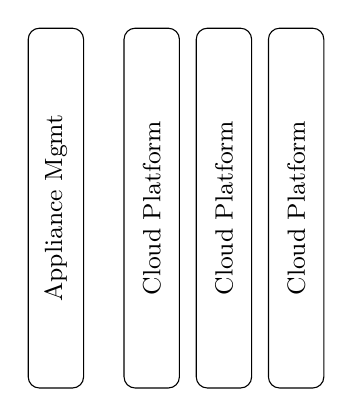
\begin{tikzpicture}[]

% cloud platform nodes
\node (cp1) [rnodesty] {\rotatebox{90}{Cloud Platform}};
\node (cp2) [rnodesty,right=0.2 of cp1] {\rotatebox{90}{Cloud Platform}};
\node (cp3) [rnodesty,right=0.2 of cp2] {\rotatebox{90}{Cloud Platform}};

\node (ap) [rnodesty,left=0.5 of cp1] {\rotatebox{90}{Appliance Mgmt}};


%\path let \p1=(s1.west),\p2=(s3.east)in
%      node (base2) [nodesty,below=0.5 of s1.south west,anchor=north west,minimum width=\x2-\x1-\pgflinewidth]
%           {base teste legal 2};

%\path let \p1=(s2.west),\p2=(s3.east) in
%      node (base3) [nodesty,above=0.5 of s2.north west,anchor=south west,minimum width=\x2-\x1-\pgflinewidth]
%           {base teste legal 3};

%\node (s4) [nodesty,left=0.25 of base3.south west,anchor=south east,minimum height=6em,minimum width=3em] {\rotatebox{90}{SVC4}};

\end{tikzpicture}
\end{document}
